
\section{层流扩散火焰}

\subsection{概述}
\subsection{无反应的恒定密度层流射流}
\subsubsection{物理描述}
无限大的容器里面充满着静止的流体(氧化剂),一股无反应的流体(燃料)喷入。

\textbf{气流核心}: 黏性力和扩散还不起作用,流体的速度和射流流体的质量分数保持不变,等于喷嘴出口的值。{\tiny 如果这个情况在管内流动那就完全不同了,根据质量守恒,显然它会加速。}

\begin{figure}[H]
    \centering
    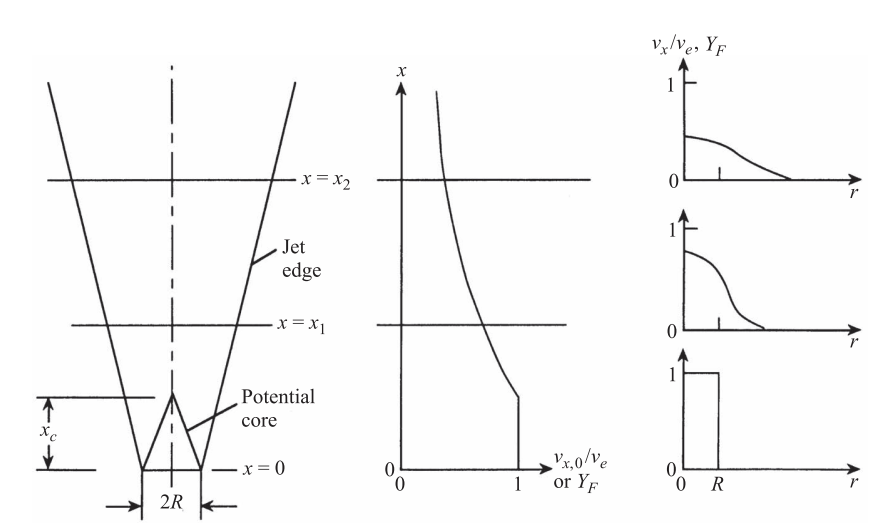
\includegraphics[width=.3\textwidth]{img/laminar_jet.png}
\end{figure}

显然存在着两个守恒:动量守恒和质量守恒,
\begin{eqnarray}
    2\pi\int_0^\infty \rho(r,x)v_x^2(r,x)r\dd r &=& \rho_e v_e^2\pi R^2\\
    2\pi\int_0^\infty \rho(r,x)v_x(r,x)Y_F(r,x)r\dd r &=& \rho_e v_e \pi R^2 Y_{F,e}
\end{eqnarray}

\subsubsection{假设}
\begin{enumerate}
    \item 射流和周围流体的摩尔质量相等。基于理想气体的性质,可以认为压力和温度都是常数,即整个流场内流体的密度为常数。
    \item 菲克扩散定律的简单二元扩散。
    \item 动量和组份扩散率为常数且相等等于1,施密特数(\(Sc\equiv \nu/\mathcal{D}\)等于1。
    \item 只考虑径向的动量和组分扩散,忽略轴向扩散。由于出口处轴向扩散很重要,所以下面的分析不适用于那里。
\end{enumerate}

\subsubsection{守恒定律}

\begin{equation}
    \begin{aligned}
        &\text{Mass:}&\frac{\pp v_x}{\pp x}+\frac{1}{r}\frac{\pp(v,r)}{\pp r}&=0\\
        &\text{Axial momentum:}& v_x \frac{\pp v_x}{\pp x}+ v_r\frac{\pp v_x}{\pp r} &= v\frac{1}{r}\frac{\pp}{\pp r}\left(r\frac{\pp v_x}{\pp r}\right)\\
        &\text{Species:}& v_x \frac{\pp Y_F}{\pp x} + v_r \frac{\pp Y_F}{\pp r}&=\mathcal{D}\frac{1}{r}\frac{\pp}{\pp r}\left(r\frac{\pp Y_F}{\pp r}\right)
    \end{aligned}
\end{equation}

那么对于氧化剂,有:
\begin{equation}
    Y_{Ox} = 1-Y_F
\end{equation}

\subsubsection{边界条件}
\begin{enumerate}
    \item 中心线的径向速度为0;
    \[v_r(0, x)=0\]
    \item 中心线的轴向速度在水平方向上变化率为0;
    \[\frac{\pp v_x}{\pp r}(0, x)=0\]
    \item 中心线的燃料质量分数在水平方向上变化率为0;
    \[\frac{\pp Y_F}{\pp r}(0, x)=0\]
    \item 轴向速度在径向的无穷远处为0;
    \[v_x(\infty, x)=0\]
    \item 燃料质量分数在径向无穷远处为0;
    \[Y_F(\infty, x) = 0\]
    \item 在出口处,速度和燃料质量分数都均匀且相等,出口外侧都为0;
    \[
        \begin{aligned}
            v_x(r\le R, 0) &=& v_e, \\
            v_x(r>R, 0) &=&0,\\
            Y_F(r\le R, 0)&=& Y_{F,e} = 1,\\
            Y_F(r>R, 0)&=&0.
        \end{aligned}
    \]
\end{enumerate}

\subsubsection{求解}
利用相似理论来进行求解,定义包含了\(r/x\)的相似变量\(\xi\)为:
\begin{equation}
    \xi = \left(\frac{3\rho_e J_e}{16\pi}\right)^{1/2}\frac{1}{\mu}\frac{r}{x}
\end{equation}

再定义初始流体动量为:
\begin{equation}
    J_e = \rho_e v_e^2\pi R^2
\end{equation}

轴向和径向速度可以表示为:
\begin{eqnarray}
    v_x &=&\frac{3}{8\pi}\frac{J_e}{\mu x}\left[1+\frac{\xi^2}{4}\right]^2\\
    v_r &=& \left(\frac{3 J_e}{16\pi\rho_e}\right)^{1/2}\frac{1}{x}\frac{\xi-\xi^3/4}{\left(1+\frac{\xi^2}{4}\right)^2}
\end{eqnarray}

我们还可以把轴向的速度写成无量纲的形式:
\begin{equation}
    v_x/v_e = 0.375(\rho_e v_e R/\mu)(x/R)^{-1}[1+\xi^2/4]^{-2}
\end{equation}
那么对于中心线的速度,代入\(\xi=0\),可以得到:
\begin{equation}
    v_{x,0}/v_e = 0.375(\rho_e v_e R/\mu)(x/R)^{-1}
\end{equation}

中间那一坨也可以写成射流雷诺数:
\begin{equation}
    Re_j \equiv \frac{\rho_e v_e R}{\mu}
\end{equation}
如前文所述,靠近喷口的地方这个式子是不合适的。

\textbf{入射流半宽}\(r_{1/2}\):在射流的某一轴向距离处,当射流速度减小到该轴向距离处中心线速度一半时的径向距离为此轴向距离处的射流半宽。
\textbf{扩张率}:射流半宽和轴向距离的比值。
\textbf{扩张角}:正切值等于扩张率的角度。
\begin{figure}[H]
    \centering
    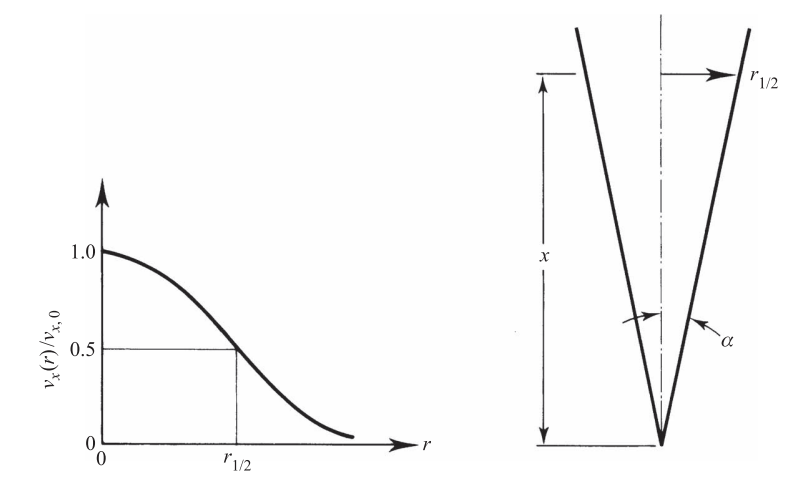
\includegraphics[width=.3\textwidth]{img/spreading_laminar.png}
\end{figure}

\begin{eqnarray}
    r_{1/2}/x &=& 2.97\left(\frac{\mu}{\rho v_e R}\right)=2.97 Re_j^{-1}\\
    \alpha &\equiv& \arctan(r_{1/2}/x)
\end{eqnarray}

对于浓度场,由于我们有施密特数等于1的假设,所以他无量纲的形式实质上和速度完全相同:
\begin{eqnarray}
    Y_F &=& 0.375 Re_j(x/R)^{-1}(1+\xi^2/4)^{-2}\\
    Y_{F,0} &=& 0.375 Re_j(x/R)^{-1}
\end{eqnarray}

上面这些式子的适用范围为:

\begin{equation}
    x/R > 0.375 Re_j
\end{equation}

\begin{enumerate}
    \item 低速射流的燃料浓度衰减到与高速射流(相差10倍)相同的值时,其轴向距离只是高速射流时的 1/10。
    \item 对于给定的燃料(\(\mu/\rho\) 为常数),燃料质量分数的空间分布只与初始的体积流量有关。
\end{enumerate}

\subsection{射流火焰的物理描述}
在流场中,燃料和氧化剂之比为化学当量的点就构成了火焰面。
对于富氧燃烧,火焰长度\(L_f\)定义为:
\begin{equation}
    \Phi(r=0, x=L_f) = 1.0
\end{equation}

\begin{itemize}
    \item 发生化学反应的区域通常是很窄的,到达顶部以前,高温区域是环状的。
    \item 按说应该考虑浮力,但是考虑到拉长之后,扩散作用也会变强,所以两个可以近似认为是抵消了。
    \item 对于圆口火焰,火焰长度和初始速度及管径都无关,粗略估算:
    \begin{equation}
        L_f\approx \frac{3}{8\pi}\frac{Q_F}{\mathcal{D}Y_\mathrm{F,stoic}}
    \end{equation}火焰长度确实是和体积流量成正比,而且还和燃料的化学当量质量分数成反比。
\end{itemize}

\subsection{简化理论描述}

\subsubsection{基本假设}

